\documentclass[14pt,mathserif,dvipdfmx,aspectratio=32]{beamer}
\usepackage{atbegshi}
\AtBeginShipoutFirst{\special{pdf:tounicode EUC-UCS2}}
%\AtBeginShipoutFirst{\special{pdf:tounicode 90ms-RKSJ-UCS2}}
\usepackage{minijs}
%\usepackage{oft}
\renewcommand{\kanjifamilydefault}{\gtdefault}
\usetheme{default}
\setbeamertemplate{navigation symbols}{}
\setbeamercolor{frametitle}{fg=black}
\setbeamercolor{title}{fg=black}
\setbeamercolor{table}{fg=black}
\setbeamersize{text margin right=0.5cm}
\setbeamersize{text margin left=0.5cm}
%\setbeamerfont{euler}
\usepackage{eulervm}


\title{サーバ仮想化の急増による問題点}
%\subtitle{すべてわかるSDN大全p90$\sim$p92}
\author[氏名略称]{原田崇司}
\institute[所属略称]{神奈川大学大学院理学研究科 情報科学専攻 田中研究室}
\date{\empty}	
%
% contents
%
\begin{document}
\begin{frame}
 \titlepage
\end{frame}
%
 \section*{内容}
 \begin{frame}{目次}
  \tableofcontents
 \end{frame}
%

\begin{frame}{高機能なアクセススイッチへ置換}


 \centering{
  \includegraphics[scale=0.8]{test.eps}
  }

\end{frame}


\begin{frame}[plain]{データプレーン構築手法}

 \centering{
  \input{test.tps}
  }

$\sum^{n}_{k=0}a_{k}$

\end{frame}

%
% \section*{references}
% \begin{frame}[allowframebreaks]{References}
%  \scriptsize
%  \bibliographystyle{jplain}
%  \bibliography{ebibtex}
% \end{frame}
 %
% \slide{ご清聴ありがとうございました.}
%
\end{document}
